\section{Plant Suitability Filtering}

When the terrain clusters have been generated, the user must specify the plant species to plot. The ecosystem simulator is then used to determine a suitable distribution for the species given the resources associated with the individual clusters.\\

Rather than permit the user to select any plant from the database with which to populate the terrain, a filtering pass is performed in order to suggest only the plants which are able to survive. To determine whether a given specie is suited, a \textit{specie suitability score} is calculated for each specie based on the resources of the given cluster. How this score is calculated is described in \textit{Calculating the Specie Suitability Score} below.\\

As well as being used to filter out ill-suited species, this suitability score also highlights the species which strive in the given environment and could, as a consequence, prove to be useful information for the user when selecting the plants species to select. Various methods are used to effectively communicate the suitability score of each specie to the user, details of which are discussed in \textit{Communicating the Suitability Score} below.

\subsection{Calculating the Specie Suitability Score}

The specie suitability score associated to a given specie \textit{S} for cluster \textit{C}, \textit{AggregateScore$_{S}$(C)}, illustrates how suited specie \textit{S} is to the environment of cluster \textit{C} on a range of 0 (ill-suited) to 100 (perfect conditions). To calculate it, the resource requirements of specie \textit{S} are matched with the resource availability of cluster \textit{C}.\\

To determine this aggregate score, it is first necessary to determine the specie's suitability to the environment in terms of \textit{slope}, \textit{illumination}, \textit{soil humidity} and \textit{temperature}. A separate score is calculated for each and is discussed separately below. 

\subsubsection{Slope Suitability Score}

The slope suitability score determines how well suited the specie is in terms of slope and is calculated as illustrated in equation \ref{eq:slope_suitability_score}.

\begin{equation}
\centering
SlopeScore_{S}(x) = 
\begin{cases}
    100, & \text{if } x \leq max \\
    0,              & \text{otherwise}
\end{cases}
\label{eq:slope_suitability_score}
\end{equation}

Where: \textit{SlopeScore$_{S}$(x)} is the slope suitability score for specie \textit{S} given slope \textit{x}; \textit{max} is the maximum slope configured for specie \textit{S}.

\subsubsection{Illumination Suitability Score}

Because the illumination varies on a monthly basis, to calculate the aggregate illumination score for a given specie is is necessary to calculate the \textit{illumination score} for each month as illustrated in equation \ref{eq:monthly_illumination_score}.

\begin{equation}
\centering
IllumScore_{S}(x) = 
\begin{cases}
    0, & \text{if } x \leq min \text{ or } x \geq max \\
    \frac{x - min}{prime_{start} - min} \times 100, & \text{if } x \in ]min,prime_{start}[ \\
    100, & \text{if } x \in [prime_{start},prime_{end}] \\
    (1 - \frac{x - prime_{end}}{max-prime_{end}}) \times 100, & \text{if } x \in ]prime_{end},max[ \\
\end{cases}
\label{eq:monthly_illumination_score}
\end{equation}
Where: \textit{IllumScore$_{S}$(x)} is the illumination suitability score for specie \textit{S} given illumination \textit{x}; \textit{min} is the minimum illumination configured for specie \textit{S};\textit{max} is the maximum illumination configured for specie \textit{S}; \textit{prime$_{start}$} is the start of the prime illumination range configured for specie \textit{S};\textit{prime$_{end}$} is the end of the prime illumination range configured for specie \textit{S}.

Given the illumination scores for each month, it is possible to calculate the \textit{average illumination score} using equation \ref{eq:avg_illumination_score}.
\begin{equation}
\centering
AvgIllumScore_{S}(x) =
\begin{cases}
	\frac{\sum_{m=1}^{m=12} IllumScore_{S}(m)}{12}, & \text{if } IllumScore_{S}(m) > 0 \text{ for } m \in [1,12] \\
    0,              & \text{otherwise}
\end{cases}
\label{eq:avg_illumination_score}
\end{equation}

\subsubsection{Humidity Suitability Score}

The humidity also varies on a monthly basis and, as such, it is also necessary to calculate the humidity score for each month as illustrated in equation \ref{eq:monthly_humidity_score}.

\begin{equation}
\centering
HumScore_{S}(x) = 
\begin{cases}
    0, & \text{if } x \leq min \text{ or } x \geq max \\
    \frac{x - min}{prime_{start} - min} \times 100, & \text{if } x \in ]min,prime_{start}[ \\
    100, & \text{if } x \in [prime_{start},prime_{end}] \\
    (1 - \frac{x - prime_{end}}{max-prime_{end}}) \times 100, & \text{if } x \in ]prime_{end},max[ \\
\end{cases}
\label{eq:monthly_humidity_score}
\end{equation}
Where: \textit{HumScore$_{S}$(x)} is the humidity suitability score for specie \textit{S} given humidity \textit{x}; \textit{min} is the minimum humidity configured for specie \textit{S}; \textit{max} is the maximum humidity configured for specie \textit{S}; \textit{prime$_{start}$} is the start of the prime humidity range configured for specie \textit{S}; \textit{prime$_{end}$} is the end of the prime humidity range configured for specie \textit{S}.

Given the humidity scores for each month, it is possible to calculate the \textit{average humidity score} using equation \ref{eq:avg_humidity_score}. 
\begin{equation}
\centering
AvgHumScore_{S}(x) =
\begin{cases}
	\frac{\sum_{m=1}^{m=12} HumScore_{S}(m)}{12}, & \text{if } HumScore_{S}(m) > 0 \text{ for } m \in [1,12] \\
    0,              & \text{otherwise}
\end{cases}
\label{eq:avg_humidity_score}
\end{equation}

\subsubsection{Temperature Suitability Score}

Temperature also varies on a monthly basis and, as such, it is also necessary to calculate the temperature score for each month as illustrated in equation \ref{eq:monthly_temp_score}.

\begin{equation}
\centering
TempScore_{S}(x) = 
\begin{cases}
    0, & \text{if } x \leq min \text{ or } x \geq max \\
    \frac{x - min}{prime_{start} - min} \times 100, & \text{if } x \in ]min,prime_{start}[ \\
    100, & \text{if } x \in [prime_{start},prime_{end}] \\
    (1 - \frac{x - prime_{end}}{max-prime_{end}}) \times 100, & \text{if } x \in ]prime_{end},max[ \\
\end{cases}
\label{eq:monthly_temp_score}
\end{equation}
Where: \textit{TempScore$_{S}$(x)} is the temperature suitability score for specie \textit{S} given temperature \textit{x};\textit{min} is the minimum temperature configured for specie \textit{S}; \textit{max} is the maximum temperature configured for specie \textit{S}; \textit{prime$_{start}$} is the start of the prime temperature range configured for specie \textit{S};  \textit{prime$_{end}$} is the end of the prime temperature range configured for specie \textit{S}.
\end{itemize}

Given the temperature scores for each month, it is possible to calculate the \textit{average temperature score} using equation \ref{eq:avg_temp_score}.

\begin{equation}
\centering
AvgTempScore_{S}(x) =
\begin{cases}
	\frac{\sum_{m=1}^{m=12} TempScore_{S}(m)}{12}, & \text{if } TempScore_{S}(m) > 0 \text{ for } m \in [1,12] \\
    0,              & \text{otherwise}
\end{cases}
\label{eq:avg_temp_score}
\end{equation}

\subsubsection{Specie Suitability Score}

The suitability score gives an overview of the specie's suitability and is calculated using equation \ref{eq:specie_suitability_score}

\begin{equation}
\begin{split}
\centering
Score_{S}(s,i,h,t) = 
\begin{cases}
	\frac{SlopeScore_{S}(s) + AvgIllumScore_{S}(i) + AvgHumScore_{S}(h) + AvgTempScore_{S}(x)}{4}, & \text{if } \\ TempScore_{S}(m) > 0 \text{ and } AvgIllumScore_{S}(m) > 0 \text{ and } \\ AvgHumScore_{S}(m) > 0 \text{ and } AvgTempScore_{S}(m) > 0 \\
    0,              & \text{otherwise}
\end{cases}
\end{split}
\label{eq:specie_suitability_score}
\end{equation}

\subsection{Communicating the Specie Suitability Score}

When all the terrain clusters have been created, the terrain suitability score for each specie in the plant database is calculated in relation to the resources of each individual cluster. If the calculated score is zero for all clusters, the specie is automatically filtered out to prevent the user from selecting it. \\

Color coding is used to make further use of the specie suitability score and intuitively communicate to the user the species most suited to the environment (see figure \ref{fig:specie_color_coding}).\\

\begin{figure}
\center
	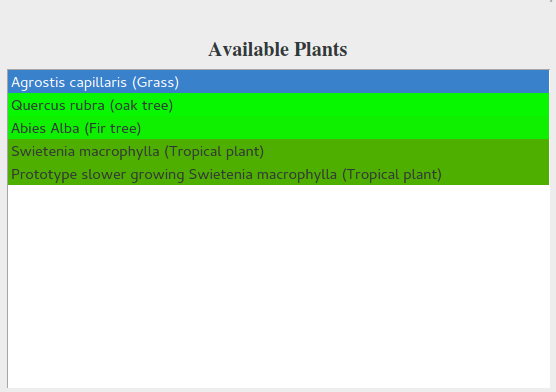
\includegraphics[width=\textwidth/2]{specie_suitability_color.png}
	\caption{ Color coding for specie suitability. The greener the highlight the more suited the specie is to the environment.}	
	\label{fig:specie_color_coding}
\end{figure}

When the user selects a given specie, all intermediate scores which were used to calculate the \textit{specie suitability score} are communicated to the user in histogram form (see figure \ref{fig:specie_intermediate_suitability_scores}).

\begin{figure}
\center
	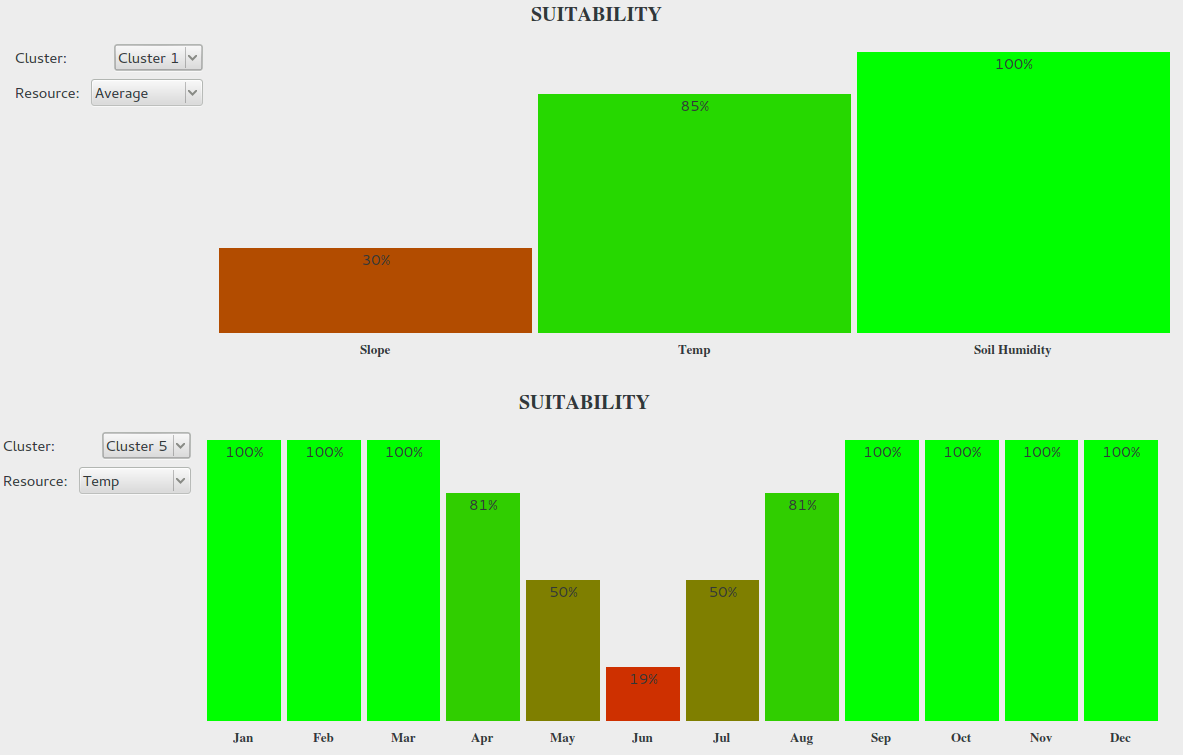
\includegraphics[width=\textwidth]{specie_suitability_temp_and_avg.png}
	\caption{ Average (top) and temperature (bottom) intermediate specie suitability histograms. Not displayed but also generated are the illumination and humidity intermediate specie suitability histograms.}	
	\label{fig:specie_intermediate_suitability_scores}
\end{figure}


